\documentclass[twoside,11pt]{article}

% Any additional packages needed should be included after jmlr2e.
% Note that jmlr2e.sty includes epsfig, amssymb, natbib and graphicx,
% and defines many common macros, such as 'proof' and 'example'.
%
% It also sets the bibliographystyle to plainnat; for more information on
% natbib citation styles, see the natbib documentation, a copy of which
% is archived at http://www.jmlr.org/format/natbib.pdf

\usepackage{jmlr2e}
\usepackage{algorithm}
\usepackage{algpseudocode}
\usepackage{listings}
\usepackage{caption}
\usepackage{amsmath}
%\usepackage[hyphens,spaces,obeyspaces]{url}

% Definitions of handy macros can go here

\newcommand{\dataset}{{\cal D}}
\newcommand{\fracpartial}[2]{\frac{\partial #1}{\partial  #2}}

\firstpageno{1}

\begin{document}

\title{Time Series Forecasting: ARIMA vs. LSTM}

\author{\name Emily Nomura \email emily\_nomura@alumni.brown.edu \\
       \addr Data Science Initiative\\
       Brown University\\
       Machine Learning: from Theory to Algorithms\\
       DATA 2060, Spring 2023\\
       }

\maketitle

\begin{abstract}%   <- trailing '%' for backward compatibility of .sty file
This paper provides a theoretical introduction to the Autoregressive Integrated Moving Average (ARIMA) and Long Short-Term Memory (LSTM) models. It compares the two models with respect to the minimization of their error rates and discusses successful applications of LSTM for time series forecasting. This paper summarizes the major findings of \textit{A Comparison of ARIMA and LSTM in Forecasting Time Series}, which was presented at the 2018 17th IEEE International Conference on Machine Learning and Applications ~\citep{siami-namini:2018}.
\end{abstract}

\begin{keywords}
  Time Series Forecasting, Deep learning, Autoregressive Integrated Moving Average (ARIMA), Long Short-Term Memory (LSTM)
\end{keywords}

\section{Introduction}
Time series forecasting is applicable in many sectors. It is most notably used in business and finance, as the  U.S. stock market is incredibly volatile. However, it also has relevance in geology (earthquake prediction), environmental science (global temperature models), and public health (disease modeling).

Given the ``big boom" of data collection in the past few decades, time series data is not difficult to acquire. Time series forecasting is applicable to any type of business, and the outcomes of interest can vary greatly in order to fit the business's needs.

When working with time series data, the most classic technique is often some type of autoregressive model, the most popular of which is the Autoregressive Integrated Moving Average (ARIMA) model. The mathematics and pseudocode for ARIMA is discussed further in \hyperref[sec:arima]{Section 2}.

Recent advances in machine learning and deep learning techniques have led to their widespread implementation in various business problems, including time series forecasting. Long Short-Term Memory (LSTM) models are reported to outperform typical time series models like ARIMA, with an average error rate reduction of 84\%-87\% \citep{siami-namini:2018}. This paper will compare ARIMA and LSTM models with respect to the minimization of their error rates as implemented by Siami-Namini et al. 

\newpage
\section{Autoregressive Integrated Moving Average (ARIMA)}
\label{sec:arima}

%\subsection{Background}
%\label{sec:arima1}
An autoregressive model contains previous values of the target variable as predictors. The lagged values can be used directly in the model, however, it is more common to incorporate differencing, which uses the difference between the lagged values as predictors. Differencing ``stabilizes" the predictors and ensures that the mean variance is stationary; a general rule of thumb in order to ensure a robust model \citep{yiu}. The benefits of differencing can be observed when comparing the variation in \hyperref[fig:gdp1]{Figure 1} to the stationarity of \hyperref[fig:gdp2]{Figure 2}.
% attach images about stationarity from TDS1
\begin{figure}[H]
    \centering
    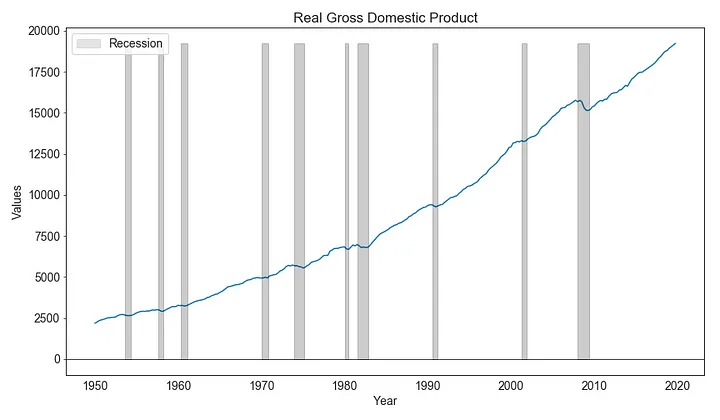
\includegraphics[scale=0.3]{img/gdp-eg1.jpeg}
    \caption{U.S. Real GDP (source: Federal Reserve Bank of St. Louis) \citep{yiu}}
    \label{fig:gdp1}
\end{figure}
\begin{figure}[H]
    \centering
    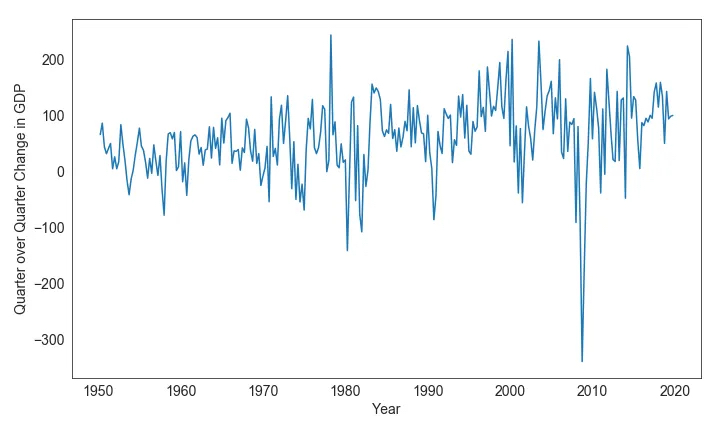
\includegraphics[scale=0.3]{img/gdp-eg2.jpeg}
    \caption{Change in Real GDP is more stationary \citep{yiu}.}
    \label{fig:gdp2}
\end{figure}

% Talk about moving average
A moving average model uses the errors of past forecasts in order to make predictions \citep{binhuraib}. This process is very similar to loss minimization, as the model is technically ``learning" from its previous errors. 

The ARIMA model combines the autoregressive model and moving average model. It incorporates differencing to forecast future values from past observations. Although an ARIMA model works well in many cases, Long Short Term Memory (LSTM) models have certain benefits over ARIMA for time series forecasting, and have gained popularity in recent years.

\subsection{Mathematics}
An autoregressive model of order $p$ and a moving average model of order $q$ can be written as in Equations \eqref{eq:Eq1} and \eqref{eq:Eq2}. 
\begin{equation}\label{eq:Eq1}
    x_t=c+\sum_{i=1}^p\phi_i x_{t-1}+\epsilon_t
\end{equation}
\begin{equation}\label{eq:Eq2}
    x_t=\mu+\sum_{i=0}^q\theta_i\epsilon_{t-i}
\end{equation}
When combined, an ARIMA model of order $(p, q)$ can be written in the following form:
\begin{equation}
    x_t=c+\sum_{i=1}^p \phi_ix_{t-i}+\epsilon_t+\sum_{i=0}^q\theta_i\epsilon_{t-1}
\end{equation}
In the ARIMA equation, $\phi_i$ represents the autocorrelation coefficients and $\theta_i$ represents the model weights. These weights are ``applied to the current and prior values of a stochastic term in the time series" \citep{siami-namini:2018}. 

In order to estimate a seasonal ARIMA model, the parameters $p$, $q$, and $d$ must be solved for. $p$ represents the number of lagged values the model takes in or the order of the autoregressive term. $q$ represents the number of previous forecast errors that the model considers or the order of the moving average term. Finally, $d$ stands for the order of differencing in the model \citep{binhuraib}. The general form of an ARIMA model is denoted $ARIMA(p, d, q)$.

\subsection{Pseudocode}
% ADD DESCRIPTION
In \textit{A Comparison of ARIMA and LSTM in Forecasting Time Series}, the authors implement a rolling ARIMA algorithm that ``performs multi-step out-of-sample forecast with re-estimation, i.e., each time the model is re-fitted to build the best estimation model" \citep{siami-namini:2018}. They fit an $ARIMA(5, 1, 0)$ model initially before iteratively re-fitting the model in order to improve upon the baseline. 
\begin{lstlisting}[frame=single]
# Rolling ARIMA
Inputs: series
Outputs: RMSE of the forecasted data
# Split data into:
# 70% training and 30% testing data
1. size=length(series) * 0.70
2. train=series[0...size]
3. test=series[size...length(size)]
# Data structure preparation
4. history=train
5. predictions=empty
# Forecast
6. for each t in range(length(test)) do
7.      model=ARIMA(history, order=(5, 1, 0))
8.      model fit=model.fit()
9.      hat=model_fit.forecast()
10.         predictions.append(hat)
11.         observed=test[t]
12.         history.append(observed)
13. end for
14. MSE = mean_squared_error(test, predictions) 
15. RMSE = sqrt(MSE)
16. Return RMSE
\end{lstlisting}

\section{Long Short-Term Memory (LSTM)}
\label{sec:lstm}

Long Short-Term Memory (LSTM) models have significant importance in the time series forecasting world due to their ability to ``remember" long-term seasonality and trends of time series data. In fact, Joos Korstanje, author of \textit{Advanced Forecasting with Python}, states \citep{keith},
\begin{quote}
    The LSTM cell adds long-term memory in an even more performant way because it allows even more parameters to be learned. This makes it the most powerful [Recurrent Neural Network] to do forecasting, especially when you have a longer-term trend in your data. LSTMs are one of the state-of-the-art models for forecasting at the moment.
\end{quote}

LSTM models are a type of deep learning model classified as a Recurrent Neural Network (RNN). The main purpose of an RNN is to predict the next step in the sequence of observations with respect to the previous steps observed in the sequence, similar to the goal of an ARIMA model \citep{siami-namini:2018}. 

The main difference between LSTM and ARIMA is the fact that LSTM is a type of neural network that consists of different ``layers" used for various learning purposes. The most basic neural network consists of three primary layer types:
\begin{enumerate}
    \item An input layer
    \item Hidden layers
    \item An output layer
\end{enumerate}

The hidden layers in an LSTM model allow it to store a great deal of information from earlier stages, usually in a sequential order, with the goal of forecasting future trends. LSTMs are composed of interconnected ``cells" or ``modules" that are used to transport and store data.

Much like a conveyor belt line in a shipping facility, LSTMs contain ``gates" where data can be disposed, filtered, or added when it is transported to the next cell in the sequence. There are three main types of gates in an LSTM \citep{siami-namini:2018}:

\begin{itemize}
    \item Forget gate. This takes on a value between $0$ and $1$ via a sigmoid activation function where $0$ tells the model to completely ignore the data and $1$ tells the model to completely remember/keep the data. The outputted values are point-wise multiplied by the previous cell state in order to determine which data should be deemed irrelevant versus relevant.
    \item Memory or input gate. This gate acts as a filter for what data should be kept. It can be described as a point-wise addition of the point-wise multiplication of two components - the output of the sigmoid layer and the output of the hyperbolic tangent layer \citep{dolphin}.
    \item Output gate. The decisions about the outputted values of each cell are made here using a sigmoid activation function. The output gate effectively ``decides" the new hidden state. The values are based on the cell state and filtered/added data.
\end{itemize}

\begin{figure}
    \centering
    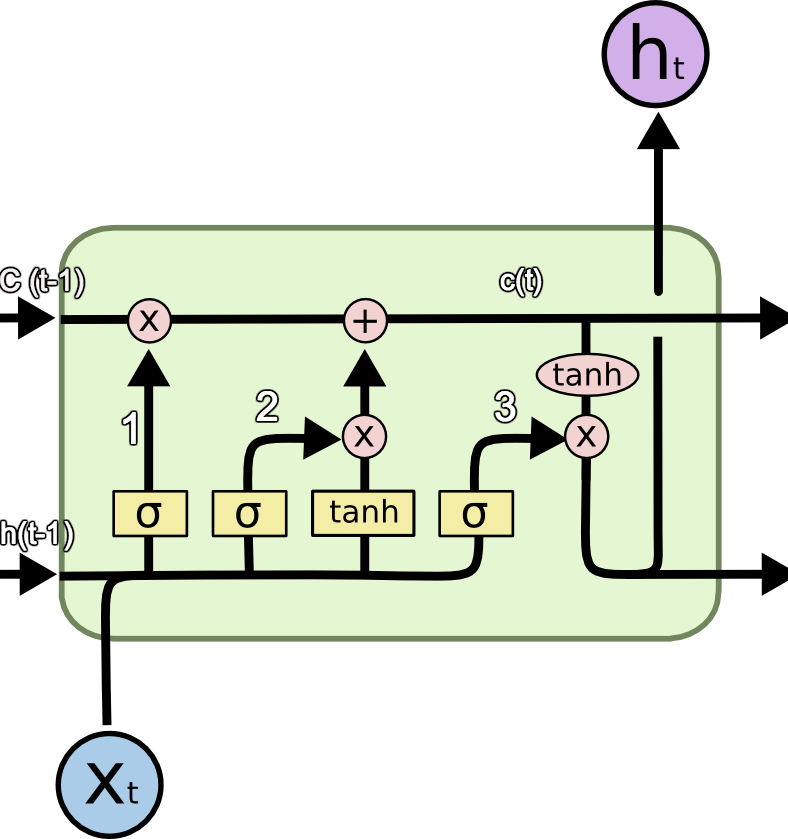
\includegraphics[scale=0.3]{img/lstm.png}
    \caption{A LSTM Unit (Source: \href{http://colah.github.io/posts/2015-08-Understanding-LSTMs}{Understanding LSTM Networks}.}
    \label{fig:lstm}
\end{figure}

\subsection{Pseudocode}
% ADD DESCRIPTION
\cite{siami-namini:2018} developed a ``multi-step univariate forecast algorithm" to implement a LSTM model for time series data. Keras and Theano packages in Python were used on a high performance computing cluster. The ``ADAM" optimization algorithm was chosen and mean squared error was specified as the loss function.
\begin{lstlisting}[frame=single]
# Rolling LSTM
Inputs: Time series
Outputs: RMSE of the forecasted data
# Split data into:
# 70% training and 30% testing data
1. size = length(series) * 0.70
2. train = series[0...size]
3. test = series[size...length(size)]
# Set the random seed to a fixed value
4. set random.seed(7)

# Fit an LSTM model to training data
Procedure fit_lstm(train, epoch, neurons)
5. X = train
6. y = train - X
7. model = Sequential()
8. model.add(LSTM(neurons), stateful=True))
9. model.compile(loss=`mean_squared_error', optimizer=`adam')
10. for each i in range(epoch) do
11.      model.fit(X, y, epochs=1, shuffle=False)
12.      model.reset_states()
13. end for
return model

# Make a one-step forecast
Procedure forecast_lstm(model, X)
14. yhat = model.predict(X)
return yhat

15. epoch = 1
16. neurons = 4
17. predictions = empty
# Fit the lstm model
18. lstm_model = fit_lstm(train,epoch,neurons)
# Forecast the training dataset
19. lstm_model.predict(train)

# Walk-forward validation on the test data
20. for each i in range(length(test)) do
21.    # make one-step forecast
22.    X = test[i]
23.    yhat = forecast_lstm(lstm_model, X)
24.    # record forecast
25.    predictions.append(yhat)
26.    expected = test[i]
27. end for
28. MSE = mean_squared_error(expected, predictions)
29. Return (RMSE = sqrt(MSE))
\end{lstlisting}

\section{Successful Applications: \cite{siami-namini:2018}}
\label{compare}
In their comparison of ARIMA vs. LSTM, \cite{siami-namini:2018} sought to answer the research question: ``Which algorithm, ARIMA or LSTM, performs more accurate prediction of time series data?"

\subsection{Dataset and Data Preparation}
\cite{siami-namini:2018} used monthly financial time series data from the Yahoo finance website between January of 1985 and August of 2018. The dataset included Nikkei 225 index (N225), NASDAQ composite index (IXIC), Hang Seng Index (HIS), S\&P 500 commodity price index (GSPC), and Dow Jones industrial average index (DJ) \citep{siami-namini:2018}. The analysis also included another dataset using economic time series data from the Federal Reserve Bank of St. Louis and the International Monetary Fund (IMF) Website.

\begin{figure}[H]
    \centering
    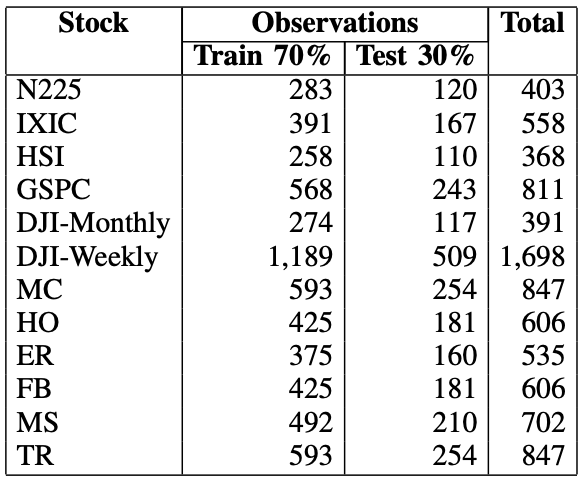
\includegraphics[scale=0.75]{img/table.png}
    \caption{The number of time series observations \citep{siami-namini:2018}.}
    \label{fig:table}
\end{figure}

The ``Adjusted Close" variable was chosen as the only financial time series feature to be utilized in the ARIMA and LSTM models. The data was split into $70\%$ training and $30\%$ testing.

\subsection{Assessment Metric}
There are many different evaluation metrics that may be used for time series forecasting. \cite{siami-namini:2018} chose to use Root-Mean-Square Error (RMSE).
\begin{equation}
    RMSE = \sqrt{\frac{1}{N}\sum_{i=1}^N (x_i-\hat{x_i})^2}
\end{equation}
$N$ represents the total number of observations in the data, $x_i$ is the true value, and $\hat{x_i}$ is the predicted value. 

\subsection{Results and Discussion}
The results of \cite{siami-namini:2018} are reported in \hyperref[fig:results]{Figure 5}. For the stock market data, the average RMSE of the Rolling ARIMA model was $511.481$ and the average RMSE of the Rolling LSTM model was $64.213$. Thus, LSTM achieved an average $87.445$ of reductions in error rates compared to ARIMA. For the economic (non-stock market) data, the average RMSE of the Rolling ARIMA model was $5.999$ and the average RMSE of the Rolling LSTM model was $0.936$. Thus, the LSTM achieved an RMSE reduction of $84.394$.

\begin{figure}[H]
    \centering
    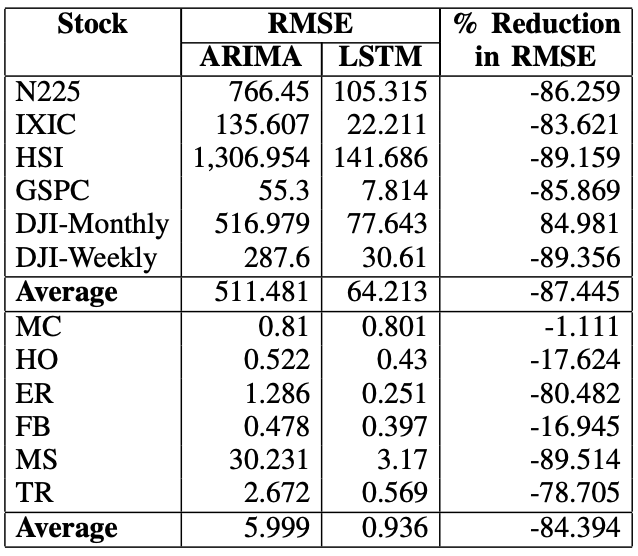
\includegraphics[scale=0.75]{img/results.png}
    \caption{The RMSEs of ARIMA and LSTM models \citep{siami-namini:2018}.}
    \label{fig:results}
\end{figure}

The LSTM model clearly outperformed the ARIMA model when implemented by \cite{siami-namini:2018} on financial and economic-related time series data. \cite{siami-namini:2018} advocates for the ``benefits of applying deep learning-based algorithms and techniques to the economics and financial data," and they hope to further investigate the improvement achieved by deep learning algorithms when compared to more traditional modeling methods.

\section{Other LSTM Applications to Time Series Data}
In addition to the application of a Rolling LSTM model to the economic and financial datasets by \cite{siami-namini:2018}, there are many other successful applications of LSTM-based models to time series forecasting, both in scholarly journals as well as online articles.

For example, Michael Keith provides a simple exploration of an LSTM model using airline data with the Python package tensorflow \citep{keith}. He was able to successfully predict the number of passengers per month using an LSTM-based model. More specifically, the model achieved a training loss of less than $0.1$ and a validation loss of less than $0.05$. After hyperparameter tuning and model selection, Keith's model outputted predictions where all but two of the points fell outside of the model's $95\%$ confidence interval.

\begin{figure}
    \centering
    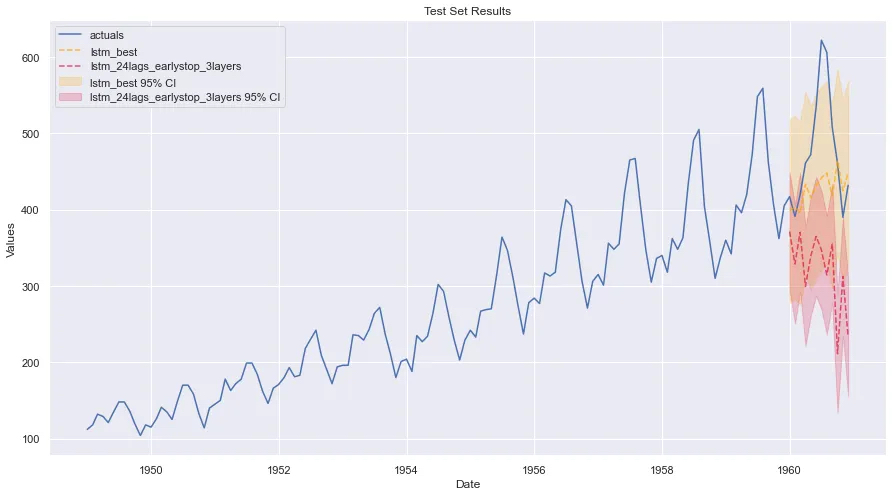
\includegraphics[scale=0.45]{img/keith.jpeg}
    \caption{LSTM Model Results on the Testing Set \citep{keith}.}
    \label{fig:keith}
\end{figure}

\section{Conclusion}
This paper provides a theoretical introduction to ARIMA and LSTM modeling techniques for time series forecasting. The methodology and findings from \textit{A Comparison of ARIMA and LSTM in Forecasting Time Series} by \cite{siami-namini:2018} are summarized. Finally, a brief synopsis of another successful application of an LSTM-based model to time series data is given.

\vskip 0.2in
\bibliography{references}

\end{document}